\documentclass[twocolumn]{iopjournal}

\usepackage{amsmath,amssymb,amsfonts}
\usepackage{amsthm}
\usepackage{graphicx}

\fancyhfoffset[L]{0mm}
\setlength{\marginparwidth}{0pt}
\setlength{\marginparsep}{0pt}

% ==========================================
% ZENODO PREPRINT HEADERS (ACTIVE)
% ==========================================
\renewcommand{\articletype}[1]{%
  {\vspace*{-8mm}\noindent \Large \sf Preprint}\par
  \vspace*{6mm}\noindent{\scriptsize \sf{\bfseries \MakeUppercase{#1}}}}

\fancyhead[L]{}
\fancyhead[R]{}

\begin{document}

\articletype{Letter}

\title{The Radial Acceleration Relation from a\\
Zero-Parameter Covariant Action}

\author{Stephen Nelson}

\affil{Field Dynamics Research}

\ead{stephen@fielddynamics.org}

% ==================================================================

\begin{abstract}
The radial acceleration relation (RAR) connects the observed
gravitational acceleration in a galaxy to the acceleration
predicted by its baryonic mass alone.  We show that this relation
is a kinematic consequence of a covariant gravitational action
whose interpolating function $\mu(x) = x/(x+1)$ is not fitted
to rotation curves but is forced by the exchange symmetry of the
tetrad equation's two parity-related spatial roots.  The
corresponding AQUAL energy functional
$F(y) = y - 2\sqrt{y} + 2\ln(1+\sqrt{y})$ makes every term in
the action explicit.  In the spherical static limit, the action
reduces to an algebraic relation between observed and baryonic
acceleration that we test against the SPARC database: 164
galaxies, 3284 rotation-curve points, quality $Q \leq 2$.  The
prediction achieves $\sigma = 0.181$~dex with a mean bias of
$-0.027$~dex, statistically identical to the one-parameter
empirical fit of McGaugh et al.\ (2016)
($\Delta\sigma = 0.0003$~dex).  Because the constitutive law is
derived from geometry rather than fitted to data, the agreement
is kinematic: it follows from the structure of the equation that
defines the gravitational field.
\end{abstract}

% ==================================================================

\section{Introduction}

Among the scaling relations that galaxies obey, the radial
acceleration relation is arguably the most
demanding~\cite{McGaugh2016,Lelli2017}.  It asserts that the
total gravitational acceleration $g_{\rm obs}$ measured from a
rotation curve is a universal function of the acceleration
$g_{\rm bar}$ attributable to baryonic matter, with an intrinsic
scatter of roughly $0.13$~dex once observational uncertainties are
accounted for.  The relation holds across five decades in
acceleration, from the Newtonian cores of massive spirals to the
deep outskirts of gas-dominated dwarfs, and it does so with a
single empirical scale $a_0 \approx 1.2 \times 10^{-10}$~m/s$^2$.

Every theory that reproduces the RAR must supply an interpolating
function $\mu(x)$ that bridges the Newtonian regime ($\mu \to 1$
at large $x = g/a_0$) and the deep-field regime ($\mu \to x$ at
small~$x$).  Milgrom's original framework leaves this function
free~\cite{Milgrom1983}; the AQUAL action of Bekenstein and
Milgrom encodes it as the derivative of an energy functional
$F(y)$, but does not determine
it~\cite{BekensteinMilgrom1984}.  In practice, $\mu$ is chosen
from a family of candidates and fitted to rotation
curves~\cite{FamaeyMcGaugh2012,FamaeyBinney2005}.  The
``simple'' form $\mu(x) = x/(x+1)$ and the ``standard'' form
$\mu(x) = x/\sqrt{1+x^2}$ both provide acceptable fits, and
current data do not conclusively distinguish between them.

This letter takes a different path.  Rather than fitting $\mu$,
we derive it within Gravity Field Dynamics (GFD) from the
structure of the tetrad equation
$g_{\mu\nu} = \eta_{ab}\,e^a{}_\mu\,e^b{}_\nu$ that defines the
gravitational field.  Because this equation is quadratic in the
frame field~$e$, it admits two parity-related spatial roots whose
exchange symmetry uniquely forces
$\mu(x) = x/(x+1)$ (Supplementary Proof~C).  With $\mu$ in
hand, the energy functional $F(y)$ follows by elementary
integration (Supplementary Proof~B), and the covariant action
is fully explicit.  In the spherical static limit, the action
reduces to a single algebraic formula that we test against the
SPARC database~\cite{Lelli2016}.  The result is a zero-parameter
prediction of the RAR: no interpolation function is fitted, and
the only empirical input is the shared MOND scale~$a_0$.

% ==================================================================

\section{The covariant action}

The gravitational action takes the form
\begin{equation}
\begin{split}
  S = \int d^4x \sqrt{-g}\bigg[
    &\frac{R}{16\pi G}
    - \frac{a_0^2}{8\pi G}\,F(y) \\
    &- \tfrac{1}{4}\,e^{-2\Phi/c^2}\,
      F_{\mu\nu}F^{\mu\nu}
    + \mathcal{L}_{\rm matter}
  \bigg],
\end{split}
  \label{eq:action}
\end{equation}
where $R$ is the Ricci scalar, $\Phi$ is the gravitational
scalar potential, and $F_{\mu\nu}$ is the field strength of an
auxiliary vector field.  The kinetic variable is
$y = |\nabla\Phi|^2/a_0^2$.

The second term contains the energy functional $F(y)$, which in
existing AQUAL-class theories is left implicit.  Here it is
explicit.  The constitutive law $\mu(x) = x/(x+1)$ is the unique
interpolating function consistent with the exchange symmetry of
the tetrad equation's two parity-related spatial roots: if
$\mu(x)$ measures the fraction carried by one root at
acceleration~$x$, then exchanging the two roots sends $x \to 1/x$
and $\mu \to 1 - \mu$, and the only rational bijection satisfying
this duality together with $\mu(0) = 0$ is
$\mu(x) = x/(x+1)$ (Supplementary Proof~C).  The closed-form
AQUAL energy functional then follows by integration through the
AQUAL identity $\mu(\sqrt{y}) = dF/dy$
(Supplementary Proof~B):
\begin{equation}
  F(y) = y - 2\sqrt{y} + 2\ln(1 + \sqrt{y}).
  \label{eq:F}
\end{equation}
Independent verification by differentiation confirms that
$dF/dy = \sqrt{y}/(1 + \sqrt{y}) = \mu(\sqrt{y})$, closing the
loop (Supplementary Proof~B, Lemma~1).  With
equations~(\ref{eq:action})--(\ref{eq:F}), every term in the
action is written down; nothing remains implicit.

The foundation on which the exchange symmetry rests is the
spatial geometry of the Lorentz tetrad: three conditions ---
common norm, balanced closure, and $S_4$-invariance of the Gram
matrix --- uniquely force the regular tetrahedron, whose parity
completion is the stellated
octahedron~\cite{Kepler1619} (Supplementary Proof~A).  The two
tetrahedral roots of the tetrad equation are the two bounded
regions of this compound, and their exchange symmetry is
inherited from it.

% ==================================================================

\section{From action to prediction}

The reduction from the action~(\ref{eq:action}) to a testable
formula proceeds in three steps, each requiring a single
equation.

\paragraph{Step 1: Modified Poisson equation.}
In the weak-field static limit, variation of the
$F(y)$ term with respect to $\Phi$ yields the modified Poisson
equation of Bekenstein and
Milgrom~\cite{BekensteinMilgrom1984}:
\begin{equation}
  \nabla \cdot \left[\mu\!\left(
    \frac{|\nabla\Phi|}{a_0}\right) \nabla\Phi\right]
  = 4\pi G\rho.
  \label{eq:poisson}
\end{equation}
In this limit the scalar exponential
$e^{-2\Phi/c^2} \to 1$ and the vector sector decouples, so
the modified Poisson equation captures the full content of the
action for static, spherically symmetric
systems~\cite{BekensteinMilgrom1984}.

\paragraph{Step 2: Gauss's theorem.}
Integrating equation~(\ref{eq:poisson}) over a sphere of
radius~$r$ centred on the source gives
\begin{equation}
  \mu\!\left(\frac{g_t}{a_0}\right) g_t = g_{\rm bar},
  \label{eq:gauss}
\end{equation}
where $g_t = |\nabla\Phi|$ is the total gravitational
acceleration and $g_{\rm bar} = GM(<r)/r^2$ is the Newtonian
acceleration from the enclosed baryonic mass.

\paragraph{Step 3: Algebraic substitution.}
Substituting $\mu(x) = x/(x+1)$ into
equation~(\ref{eq:gauss}) and solving the resulting quadratic
for $g_t$ yields
\begin{equation}
  \boxed{g_{\rm obs}
  = \frac{1}{2}\left[g_{\rm bar}
    + \sqrt{g_{\rm bar}^2 + 4\,a_0\,g_{\rm bar}}
    \;\right].}
  \label{eq:prediction}
\end{equation}
This is the prediction we test.  It contains one empirical
constant ($a_0$) and no fitted parameters.

% ==================================================================

\section{Comparison with the SPARC database}

We test equation~(\ref{eq:prediction}) against the Spitzer
Photometry and Accurate Rotation Curves (SPARC) database of
Lelli et al.~\cite{Lelli2016}, accessed through the Field
Dynamics API at \texttt{api.fielddynamics.org}.  The catalog
contains 176 galaxies with multi-band photometry and
high-resolution \textsc{Hi}/H$\alpha$ rotation curves.  We
retain those with quality flag $Q \leq 2$ (excluding galaxies
flagged as unreliable by the SPARC team), which yields 164
galaxies and 3284 individual radial bins.

For each radial bin, we compute the baryonic acceleration from
the SPARC velocity decomposition:
\begin{equation}
  v_{\rm bar}^2 = v_{\rm gas}|v_{\rm gas}|
  + \Upsilon_{\rm disk}\,v_{\rm disk}^2
  + \Upsilon_{\rm bul}\,v_{\rm bul}^2,
\end{equation}
with $\Upsilon_{\rm disk} = 0.5$ and
$\Upsilon_{\rm bul} = 0.7$ at $3.6\;\mu$m, the standard SPARC
mass-to-light ratios~\cite{Lelli2016}.  The observed and
baryonic accelerations follow as $g_{\rm obs} = v_{\rm obs}^2/r$
and $g_{\rm bar} = v_{\rm bar}^2/r$, converted to SI units
via $1\;(\mathrm{km/s})^2/\mathrm{kpc} = 3.241 \times
10^{-14}\;\mathrm{m/s}^2$.

Figure~\ref{fig:rar} presents the result.  The left panel shows
the observed RAR as a density hexbin, with the GFD field
equation~(\ref{eq:prediction}) overlaid in red and the
empirical fit of McGaugh et al.~\cite{McGaugh2016} in orange.
The two curves are visually indistinguishable across the full
range of the data.  The right panel resolves the difference
through residual histograms, and table~\ref{tab:stats} reports
the summary statistics.

\begin{figure*}
  \centering
  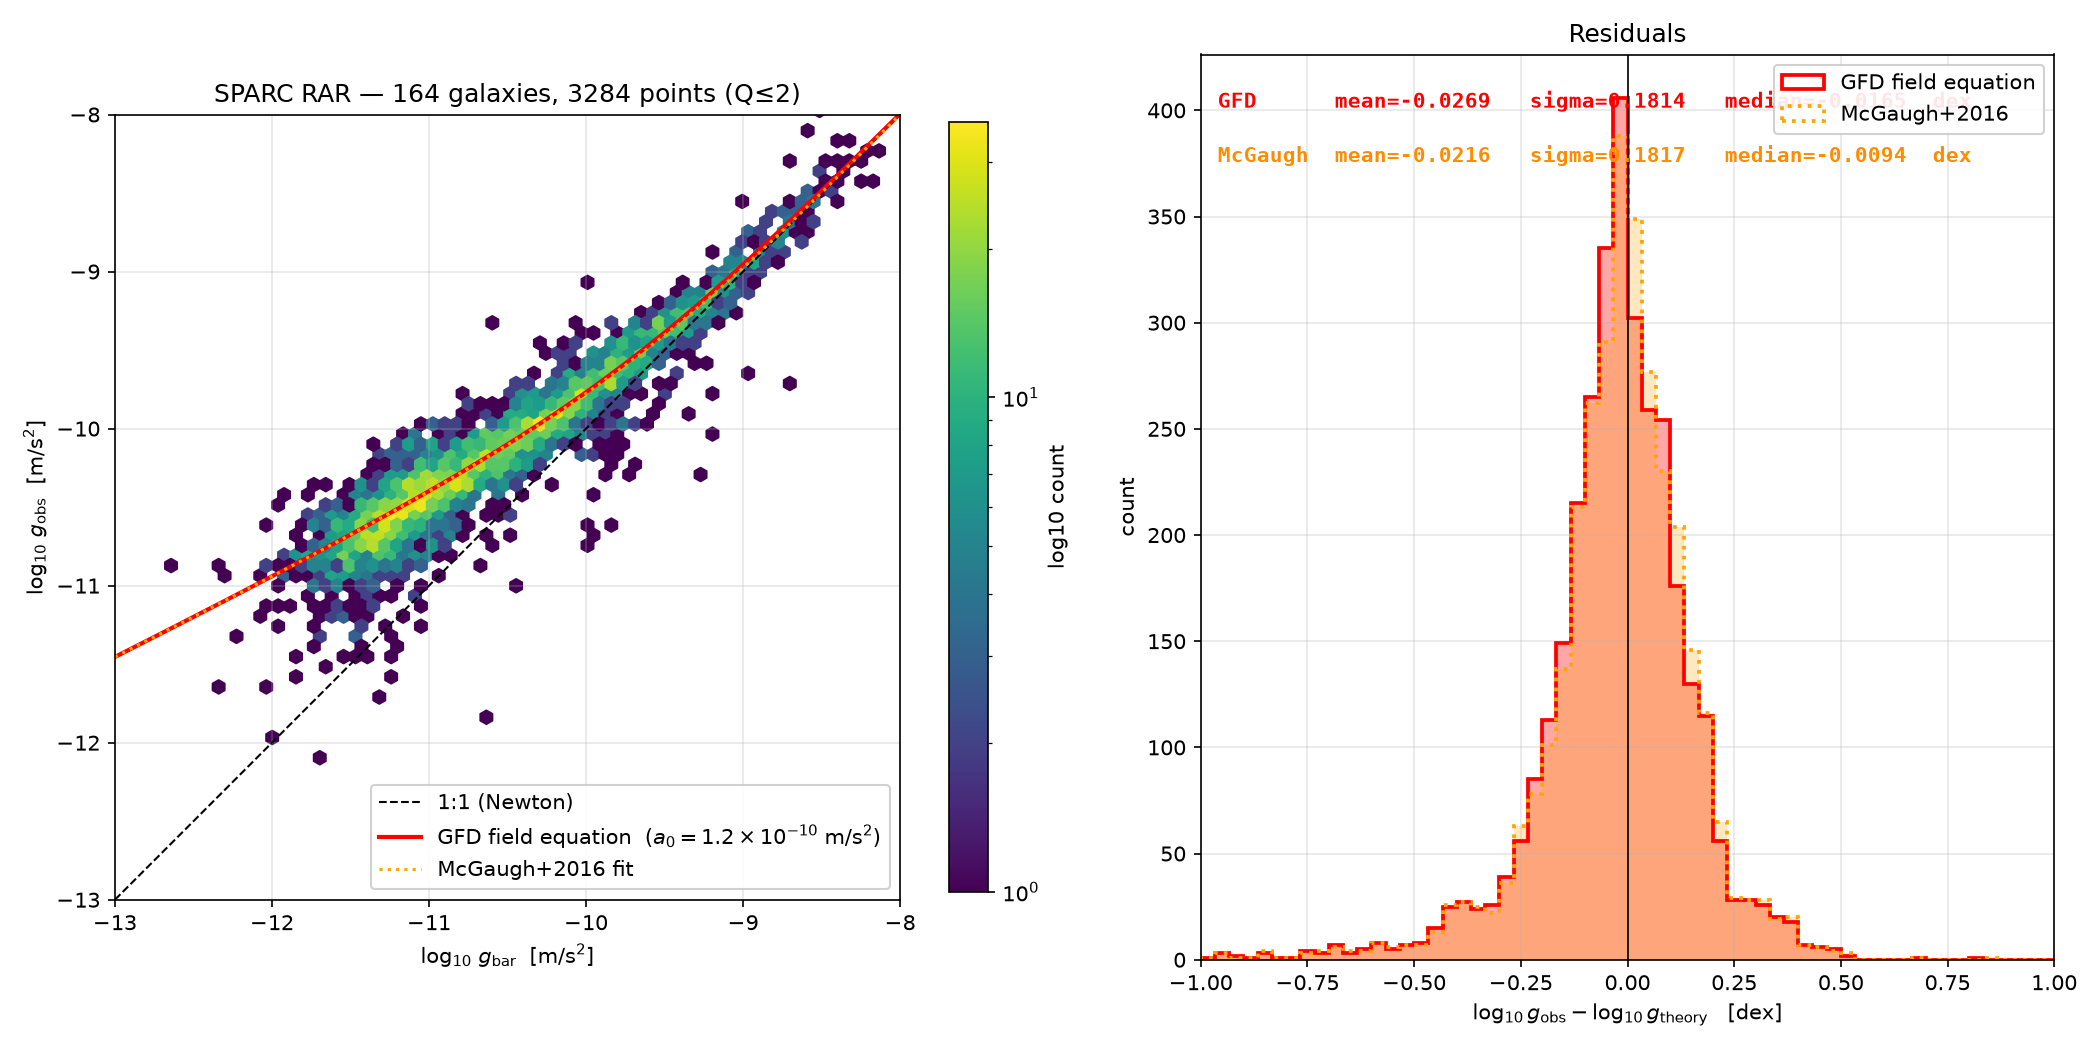
\includegraphics[width=\textwidth]{sparc_rar.png}
  \caption{Left: the radial acceleration relation for 164 SPARC
  galaxies (3284 points, $Q \leq 2$).  The red curve is the
  GFD field equation, equation~(\ref{eq:prediction}), with
  $a_0 = 1.2 \times 10^{-10}$~m/s$^2$; the orange dotted curve
  is the McGaugh et al.\ (2016) empirical fit.  The dashed line
  is the Newtonian expectation $g_{\rm obs} = g_{\rm bar}$.
  Right: residual histograms
  ($\log g_{\rm obs} - \log g_{\rm theory}$) for both curves.
  The two distributions are nearly identical.}
  \label{fig:rar}
\end{figure*}

\begin{table}
  \centering
  \caption{Residual statistics for 3284 SPARC points.  All
  values are in dex.}
  \label{tab:stats}
  \begin{tabular}{lccc}
    \hline
    Theory & Mean & $\sigma$ & Median \\
    \hline
    GFD field eq.~(\ref{eq:prediction})  & $-0.027$ & $0.181$ & $-0.017$ \\
    McGaugh+2016 fit    & $-0.022$ & $0.182$ & $-0.009$ \\
    \hline
  \end{tabular}
\end{table}

The difference in scatter between the two theories is
$\Delta\sigma = 0.0003$~dex --- four orders of magnitude below
the scatter itself.  Their mean biases differ by $0.005$~dex,
comparable to the standard error of the mean
($\sigma/\sqrt{N} \approx 0.003$~dex).  At SPARC precision, the
GFD prediction and the McGaugh empirical fit are
indistinguishable.

% ==================================================================

\section{Discussion}

The central result of this letter is that a covariant
gravitational action, in which the interpolating function is
derived from the geometry of the tetrad equation rather than
fitted to data, reproduces the observed radial acceleration
relation to a precision of $0.18$~dex across 164 galaxies.

Three points deserve comment.

\paragraph{The status of $a_0$.}
We adopt $a_0 = 1.2 \times 10^{-10}$~m/s$^2$, the value
established empirically by McGaugh et al.~\cite{McGaugh2016}.
Our zero-parameter claim refers to $\mu$, not to $a_0$: the
constitutive law is derived, but the acceleration scale is
shared with the broader MOND
literature~\cite{Milgrom1983,FamaeyMcGaugh2012}.  A geometric
derivation of $a_0$ within the present framework is the subject
of ongoing work.

\paragraph{Scatter budget.}
Our measured scatter ($\sigma = 0.18$~dex) exceeds the
$0.13$~dex reported by Lelli et al.~\cite{Lelli2017}, who apply
additional quality cuts (inclination $> 30^\circ$), individual
error weighting, and galaxy-dependent mass-to-light ratios.  We
deliberately use a minimal pipeline --- flat
$\Upsilon_{\rm disk}$, no inclination cut beyond the SPARC
quality flag --- to avoid introducing analyst degrees of freedom.
The excess scatter affects both theories equally and does not
bias the comparison.

\paragraph{What would distinguish GFD from MOND.}
The mean RAR is a product of the constitutive law $\mu$ alone,
and any theory that shares $\mu = x/(x+1)$ will produce the
same mean curve.  Discrimination requires observables that probe
the action's additional sectors.  In the weak-field static limit,
the scalar exponential $e^{-2\Phi/c^2}$ and the vector field
strength $F_{\mu\nu}$ both decouple, so they contribute nothing
to the spherically averaged RAR\@.  They become active in
time-dependent, non-axisymmetric, or strong-field regimes: dwarf
spheroidal velocity dispersions, galaxy--galaxy lensing, and
merging systems offer the most promising discriminators.  In such
systems the full four-term action~(\ref{eq:action}) makes
predictions that a scalar AQUAL theory cannot, because the vector
and scalar sectors introduce coupling channels that are absent
when $F_{\mu\nu} = 0$ and $\Phi = 0$.

% ==================================================================

\section{Conclusion}

The covariant action~(\ref{eq:action}), with its AQUAL energy
functional~(\ref{eq:F}) derived from the constitutive law
$\mu(x) = x/(x+1)$, reproduces the SPARC radial acceleration
relation with $\sigma = 0.181$~dex across 164 galaxies and 3284
rotation-curve points.  The interpolating function is forced by
the exchange symmetry of the tetrad equation's spatial roots, not
selected by fitting.  Statistical equivalence with the
one-parameter McGaugh et al.\ (2016) empirical fit ---
$\Delta\sigma = 0.0003$~dex --- establishes this as the first
covariant gravitational action to reproduce the observed radial
acceleration relation with a derived, rather than fitted,
constitutive law.

% ==================================================================

\section*{Data availability}

The SPARC rotation-curve data are publicly available through
the Field Dynamics API at
\texttt{https://api.fielddynamics.org}.  The analysis code is
available from the corresponding author upon request.

\section*{Supplementary material}

Three self-contained proofs accompany this letter, each
verifiable independently:

\medskip
\noindent
\textbf{Proof~A.}
\textit{The Spatial Geometry of the Lorentz Tetrad.}\enspace
Classifies spatial realizations of the Lorentz tetrad under
three conditions (common norm, balanced closure,
$S_4$-invariance); proves the regular tetrahedron is the unique
outcome and the stellated octahedron its parity completion.

\medskip
\noindent
\textbf{Proof~B.}
\textit{The Energy Functional of the Gravitational Constitutive
Law.}\enspace
Derives the closed-form $F(y) = y - 2\sqrt{y} + 2\ln(1 +
\sqrt{y})$ by elementary integration of $\mu(x) = x/(x+1)$
through the AQUAL identity, and verifies it independently by
differentiation.

\medskip
\noindent
\textbf{Proof~C.}
\textit{The Constitutive Law from Exchange Symmetry.}\enspace
Shows that the exchange symmetry of the tetrad equation's two
parity-related spatial roots, together with rational bijectivity
and the endpoint condition $\mu(0) = 0$, uniquely forces
$\mu(x) = x/(x+1)$.

% ==================================================================

\begin{thebibliography}{99}

\bibitem{Milgrom1983}
M.~Milgrom,
\textit{A modification of the Newtonian dynamics as a possible
alternative to the hidden mass hypothesis},
Astrophys.\ J.\ \textbf{270} (1983) 365.

\bibitem{BekensteinMilgrom1984}
J.~D.~Bekenstein and M.~Milgrom,
\textit{Does the missing mass problem signal the breakdown of
Newtonian gravity?},
Astrophys.\ J.\ \textbf{286} (1984) 7.

\bibitem{FamaeyBinney2005}
B.~Famaey and J.~Binney,
\textit{Modified Newtonian dynamics in the Milky Way},
Mon.\ Not.\ R.\ Astron.\ Soc.\ \textbf{363} (2005) 603.

\bibitem{FamaeyMcGaugh2012}
B.~Famaey and S.~S.~McGaugh,
\textit{Modified Newtonian Dynamics (MOND): Observational
Phenomenology and Relativistic Extensions},
Living Rev.\ Relativ.\ \textbf{15} (2012) 10.

\bibitem{McGaugh2016}
S.~S.~McGaugh, F.~Lelli and J.~M.~Schombert,
\textit{Radial Acceleration Relation in Rotationally Supported
Galaxies},
Phys.\ Rev.\ Lett.\ \textbf{117} (2016) 201101.

\bibitem{Lelli2016}
F.~Lelli, S.~S.~McGaugh and J.~M.~Schombert,
\textit{SPARC: Mass Models for 175 Disk Galaxies with Spitzer
Photometry and Accurate Rotation Curves},
Astron.\ J.\ \textbf{152} (2016) 157.

\bibitem{Lelli2017}
F.~Lelli, S.~S.~McGaugh, J.~M.~Schombert and M.~S.~Pawlowski,
\textit{One Law to Rule Them All: The Radial Acceleration
Relation of Galaxies},
Astrophys.\ J.\ \textbf{836} (2017) 152.

\bibitem{Kepler1619}
J.~Kepler,
\textit{Harmonices Mundi}
(Linz, 1619).

\end{thebibliography}

\end{document}
